% \iffalse meta-comment
%
% Copyright (C) 2018--2023 by Xiangdong Zeng <xdzeng96@gmail.com>
% Copyright (C) 2025 by Shi Liu <sliutheory@outlook.com>
%
% This work may be distributed and/or modified under the
% conditions of the LaTeX Project Public License, either
% version 1.3c of this license or (at your option) any later
% version. The latest version of this license is in:
%
%   https://www.latex-project.org/lppl.txt
%
% and version 1.3c or later is part of all distributions of
% LaTeX version 2008 or later.
%
% This work has the LPPL maintenance status `maintained'.
%
% The Current Maintainer of this work is Shi Liu <sliutheory@outlook.com>.
%
% This work is a derived work based on the fduthesis template
% originally developed by Xiangdong Zeng.
%
% \fi
%*********************************************************************
% wuthesis: 西湖大学论文模板
% 2025-12-16 v0.1
%
% 重要提示：
%   1. 请确保使用 UTF-8 编码保存
%   2. 请使用 XeLaTeX 或 LuaLaTeX 编译
%   3. 请仔细阅读用户文档
%   4. 修改、使用、发布本文档请务必遵循 LaTeX Project Public License
%   5. 不需要的注释可以尽情删除
%*********************************************************************
\documentclass[type=proposal]{wuthesis}
%\PassOptionsToPackage{url=false, doi=false, isbn=false, eprint=false}{biblatex}
\wusetup{
  style = {
    % font = times,
    % 西文字体（包括数学字体）
    % 允许选项：
    % font = garamond|libertinus|lm|palatino|times|times*|none
    %
    % cjk-font = fandol,
    % 中文字体
    % 允许选项：
    %   cjk-font = adobe|fandol|founder|mac|sinotype|sourcehan|windows|none
    %
    % 注意：
    %   1. 中文字体设置高度依赖于系统。各系统建议方案：
    %        windows：cjk-font = windows
    %        mac：    cjk-font = mac
    %        linux：  cjk-font = fandol（默认值）
    %   2. 除 fandol 和 sourcehan 外，其余字体均为商用字体，请注意版权问题
    %   3. 但 fandol 字体缺字比较严重，而 sourcehan 没有配备楷体和仿宋体
    %   4. 这里中西文字体设置均注释掉了，即使用默认设置：
    %        font     = times
    %        cjk-font = fandol
    %   5. 使用 font = none / cjk-font = none 关闭默认字体设置，需手动进行配置
    %
    % font-size = -4,
    % 字号
    % 允许选项：
    %   font-size = -4|5
    %
    % fullwidth-stop = catcode,
    % 是否把全角实心句点 “．” 作为默认的句号形状
    % 允许选项：
    %   fullwidth-stop = catcode|mapping|false
    % 说明：
    %   catcode   显式的 “。” 会被替换为 “．”（e.g. 不包括用宏定义保存的 “。”）
    %   mapping   所有的 “。” 会被替换为 “．”（使用 LuaLaTeX 编译则无效）
    %   false     不进行替换
    %
    footnote-style = xits,
    % 脚注编号样式
    % 允许选项：
    %   footnote-style = plain|libertinus|libertinus*|libertinus-sans|
    %                    pifont|pifont*|pifont-sans|pifont-sans*|
    %                    xits|xits-sans|xits-sans*
    % 默认与西文字体保持一致
    %
    % hyperlink = color,
    % 超链接样式
    % 允许选项：
    %   hyperlink = border|color|none
    %
    % hyperlink-color = default,
    % 超链接颜色
    % 允许选项：
    %   hyperlink-color = default|classic|material|graylevel|prl
    %
    bib-backend = biblatex,
    % 参考文献支持方式
    % 允许选项：
    %   bib-backend = bibtex|biblatex
    %
    bib-style = gb7714-2015,
    % 参考文献样式
    % 允许选项：
    %   bib-style = author-year|numerical|<其他样式>
    % 说明：
    %   author-year  著者—出版年制
    %   numerical    顺序编码制
    %   <其他样式>   使用其他 .bst（bibtex）或 .bbx（biblatex）格式文件
    %
    % cite-style = {},
    % 引用样式
    % 默认为空，即与参考文献样式保持一致
    % 仅适用于 biblatex；如要填写，需保证相应的 .cbx 格式文件能被调用
    %
    bib-resource = {proposal.bib},
    % 参考文献数据源
    % 可以是单个文件，也可以是用英文逗号 “,” 隔开的一组文件
    % 如果使用 biblatex，则必须明确给出 .bib 后缀名
    %
    % logo = {fudan-name.pdf},
    % 封面中的校名图片
    % 模版已自带，通常不需要额外配置
    %
    % logo-size = {0.5\textwidth},      % 只设置宽度
    % logo-size = {{}, 3cm},            % 只设置高度
    % logo-size = {8cm, 3cm},           % 设置宽度和高度
    % 设置校名图片的大小
    % 通常不需要调整
    %
    % declaration-page = {declaration.pdf},
    % 插入扫描版的声明页 PDF 文档
    % 默认使用预定义的声明页，但不带签名
    %
    % auto-make-cover = true
    % 是否自动生成论文封面（封一）、指导小组成员名单（封二）和声明页（封三）
    % 除非特殊需要（e.g. 不要封面），否则不建议设为 false
  },
  info = {
    title = {非绝热重整化群\\在强关联电子体系中的应用
},
    author = {张三},
    student-id = {2022xxxxxxx},
    department = {理学院},
    major = {物理学},
    supervisor = {李四\quad 教授/研究员},
  }
}

% 需要的宏包可以自行调用
\usepackage{physics}

% 需要的命令可以自行定义
\newcommand{\hilbertH}{\symcal{H}}
\newcommand{\ee}{\symrm{e}}
\newcommand{\ii}{\symrm{i}}


\begin{document}


\tableofcontents
\mainmatter
% 建议采用多文件编译的方式
% 比较好的做法是把每一章放进一个单独的 tex 文件里，并在这里用 \include 导入，例如
%   \include{chapter1}
%   \include{chapter2}
%   \include{chapter3}
\chapter{文献综述}
\begin{refsection}
  \section{背景介绍}
  强关联电子体系的精确描述一直是凝聚态物理与量子化学领域的核心难题。由于多体波函数所在的希尔伯特空间随体系增大呈指数级增长，传统的精确对角化方法无法处理宏观体系，而基于平均场近似的方法又无法捕捉电子关联效应。为了在保留电子关联效应的基础上应对指数级增大的希尔伯特空间，物理学家发展了重整化群（Renormalization Group, RG）理论，旨在通过系统性的希尔伯特空间截断来提取低能有效物理。
  \begin{figure}[htb]
    \centering
    % 注意：这里的文件名需要和你实际保存的图片文件名一致
    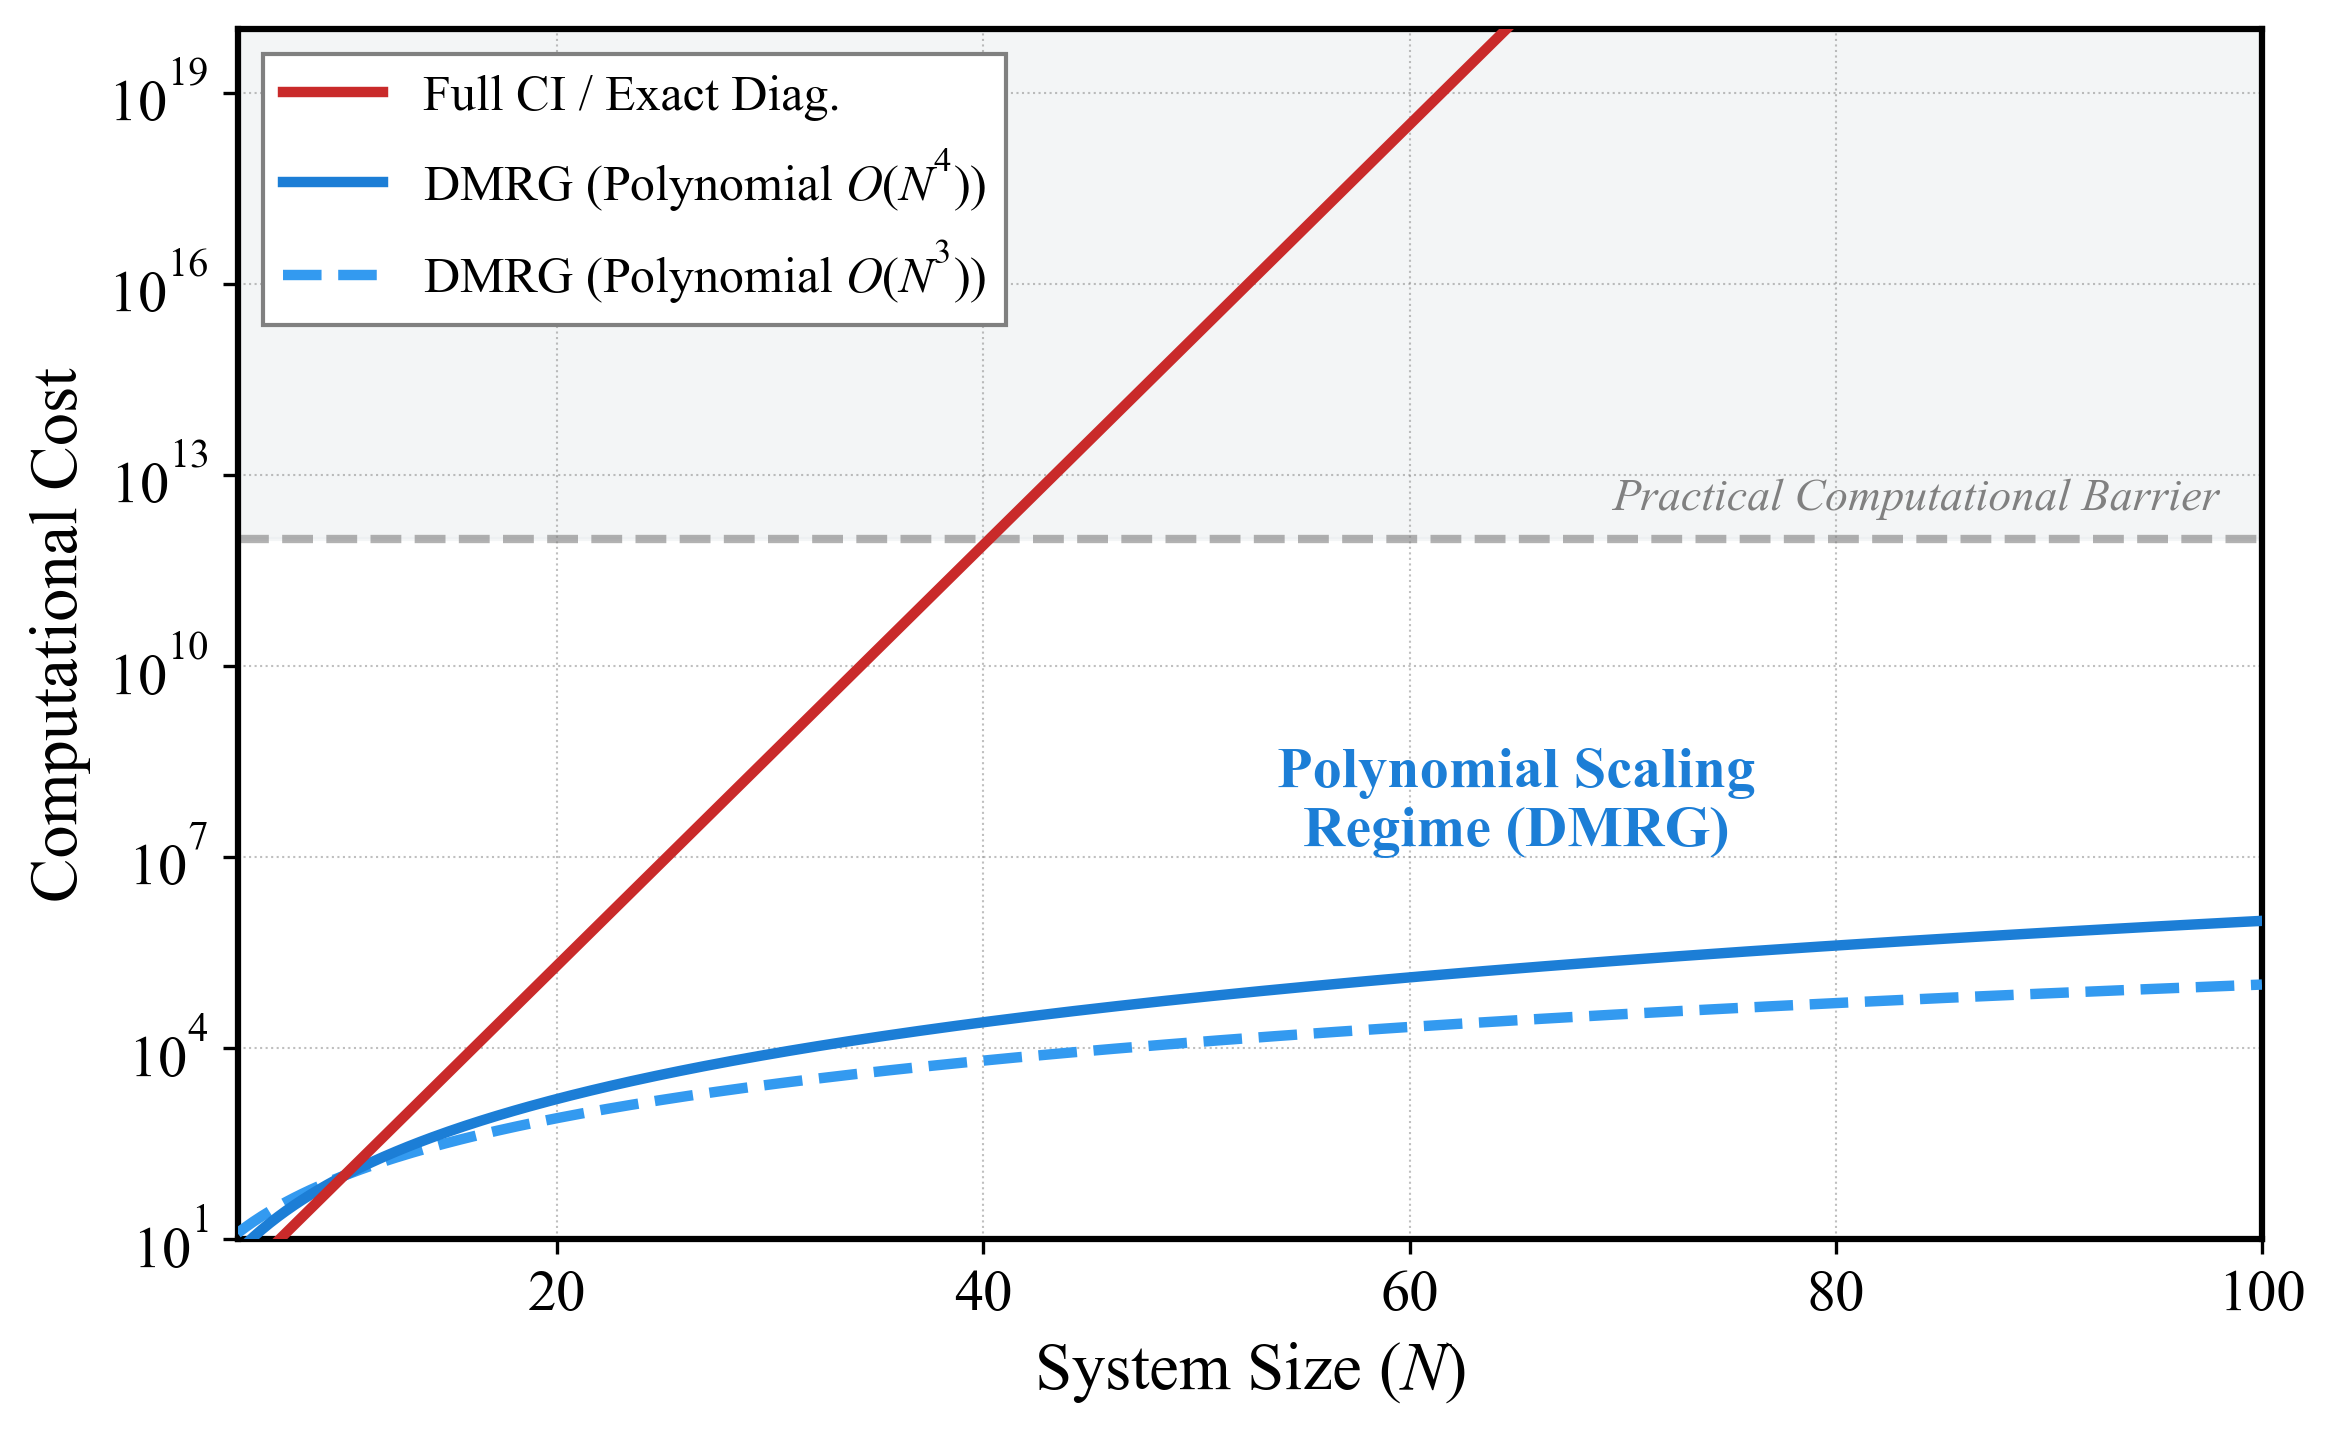
\includegraphics[width=0.8\textwidth]{fig/example_image_1.png} 
    \caption[量子多体模拟中的“指数墙”问题]{%
      量子多体模拟中的“指数墙”问题与 DMRG 算法的突破。
      图中展示了随着系统尺寸 $N$ 的增加，不同计算方法的计算代价（对数坐标）。
      红色曲线代表全组态相互作用（Full CI）或精确对角化方法，受限于希尔伯特空间的指数级爆炸，其计算量迅速触及当前硬件资源的物理极限（灰色虚线）。
      蓝色曲线展示了密度矩阵重整化群（DMRG）算法，该方法通过保留重要的低能有效状态，将计算复杂度降低为多项式级别（$O(N^3)$ 至 $O(N^4)$），从而使得对大尺度强关联体系的精确求解成为可能。}
    \label{fig:exponential_wall}
  \end{figure}
  
  文献综述部分我们将梳理本课题的理论脉络。我们首先描述强关联系统的物理特点及平均场理论的局限性，随后回顾重整化群方法从Wilson的数值重整化群（NRG）到White的密度矩阵重整化群（DMRG）的发展过程，重点讨论截断标准的转变；最后，针对将DMRG算法应用于三维量子化学体系时面临的几何映射难题，引出基于离散变量表象的基组构建策略，这也是本工作的技术路线起点。
  \subsection{强关联电子系统与平均场理论的失效}
  无论是为了解释凝聚态物理中的新奇量子物态，还是为了阐明量子化学中的微观反应机理，多体薛定谔方程的求解都是串联量子力学原理与宏观物理现象的核心。但由于电子之间存在长程的库仑相互作用，精确求解多体波函数极其困难。作为标准的出发点，平均场理论（Mean-Field Theory，如Hartree-Fock方法或传统的密度泛函理论DFT）采用单粒子近似，假设每个电子仅在由原子核和其他所有电子产生的“平均势场”中运动。这种近似下，体系的多体波函数被简化为单个Slater Determinant。尽管这一方法在描述半导体能带结构和弱关联分子的平衡构型方面取得了成功，但这种单粒子图像无法捕捉电子之间的量子关联信息，特别是当体系存在多个近简并低能态时，它无法描述电子在不同组态间的相干叠加。这种被忽略的相互作用被称为电子关联（Electron Correlation）。形式上，电子关联定义为精确的非相对论基态能量与Hartree-Fock极限能量之差：
  \begin{equation}
    E_{corr} = E_{exact} - E_{HF}
  \end{equation}
  根据背后的物理机制，电子关联通常被划分为动态关联（Dynamic Correlation）与静态关联（Static Correlation，或强关联）。动态关联源于电子间的库仑排斥，表现为电子在位置空间上存在瞬时避让，可以通过微扰论或耦合簇等方法进行修正。然而，在体系存在多个能量相近的电子组态时，起主导作用的往往是静态关联。此时单一的Slater Determinant完全失效，波函数表现为多个电子组态的强量子叠加。此时，平均场理论不再仅仅是精度不够，而是会给出定性错误的物理图像。
  平均场理论在强关联体系中的失效广泛地体现在物理及化学现象中。例如凝聚态物理中的Mott Insulators问题：根据基于平均场的能带理论，具有半满能带的过渡金属氧化物（如高温超导体母体 $La_{2}CuO_{4}$）应表现为金属；然而实验表明，由于电子间极强的库仑排斥能超过了动能，电子被迫局域在格点上，使材料转变为绝缘体\cite{Imada1998Metal}。……
  \subsection{更低一级的标题}
  正文内容
  \section{国内外研究现状}

  \subsection{研究方向及进展}
  正文内容
  \subsection{存在问题}
  正文内容
  \section{研究展望}
  正文内容
  % 以下为自动生成的文献综述中的参考文献部分
  \printbibliography[heading=bibintoc, title={参考文献}]

\end{refsection}
\chapter{开题报告}
  \begin{refsection}

  \section{问题提出的背景}
  \subsection{背景介绍}
  正文内容
  \subsubsection{更低一级的标题}
  在先前对于氢链的研究中我们观察到，如果仅仅依赖于传统的Hartree Fock方法和基于核吸引势的分子轨道初始猜测，我们需要在每个DVR切片上保留多个分子轨道才能较为精确的描述电子结构\cite{doi:10.1021/acs.jctc.5c00029}。本研究希望再此基础上进行优化，使我们可以用更少的分子轨道精确描述电子结构，为后续应用重整化群算法提供更近理想的输入。
  \subsection{本研究的意义和目的}
  正文内容
  \section{论文的主要内容和技术路线}
  \subsection{主要研究内容}
  \subsubsection{更低一级的标题}
  正文内容
  \subsubsection{更低一级的标题}
  正文内容
  \subsection{技术路线}
  \subsubsection{更低一级的标题}
  正文内容
  \subsubsection{更低一级的标题}
  正文内容
  \subsection{可行性分析}
  本研究建立在凝聚态物理与量子化学领域成熟的理论基石之上。Hybrid Gaussian/DVR 基组的构建是基于Steven White等人提出的Sliced Basis理论。同时，非绝热重整化群条件本征化的核心思想在物理上是清晰的。

  目前已完成了初步的基组构建与哈密顿量生成的代码开发工作。我们已推导并实现了混合表象下的动能、势能及双电子库仑积分公式，通过在不同区间分别采用数值计算与Prony拟合的方法，能够处理1/r奇异性问题。而针对基组优化环节，我们已完成了Hartree-Fock能量函数关于基组缩并系数的解析Gradient与Hessian的数学推导。初步的数值测试表明，基于牛顿法的扫描优化策略具有良好的收敛性。后续工作主要集中在此算法的优化，DMRG的实现，以及重整化群逻辑的组装与物理应用上。
  \begin{figure}[htb]
    \centering
    % 请确保文件名与你实际保存的一致
    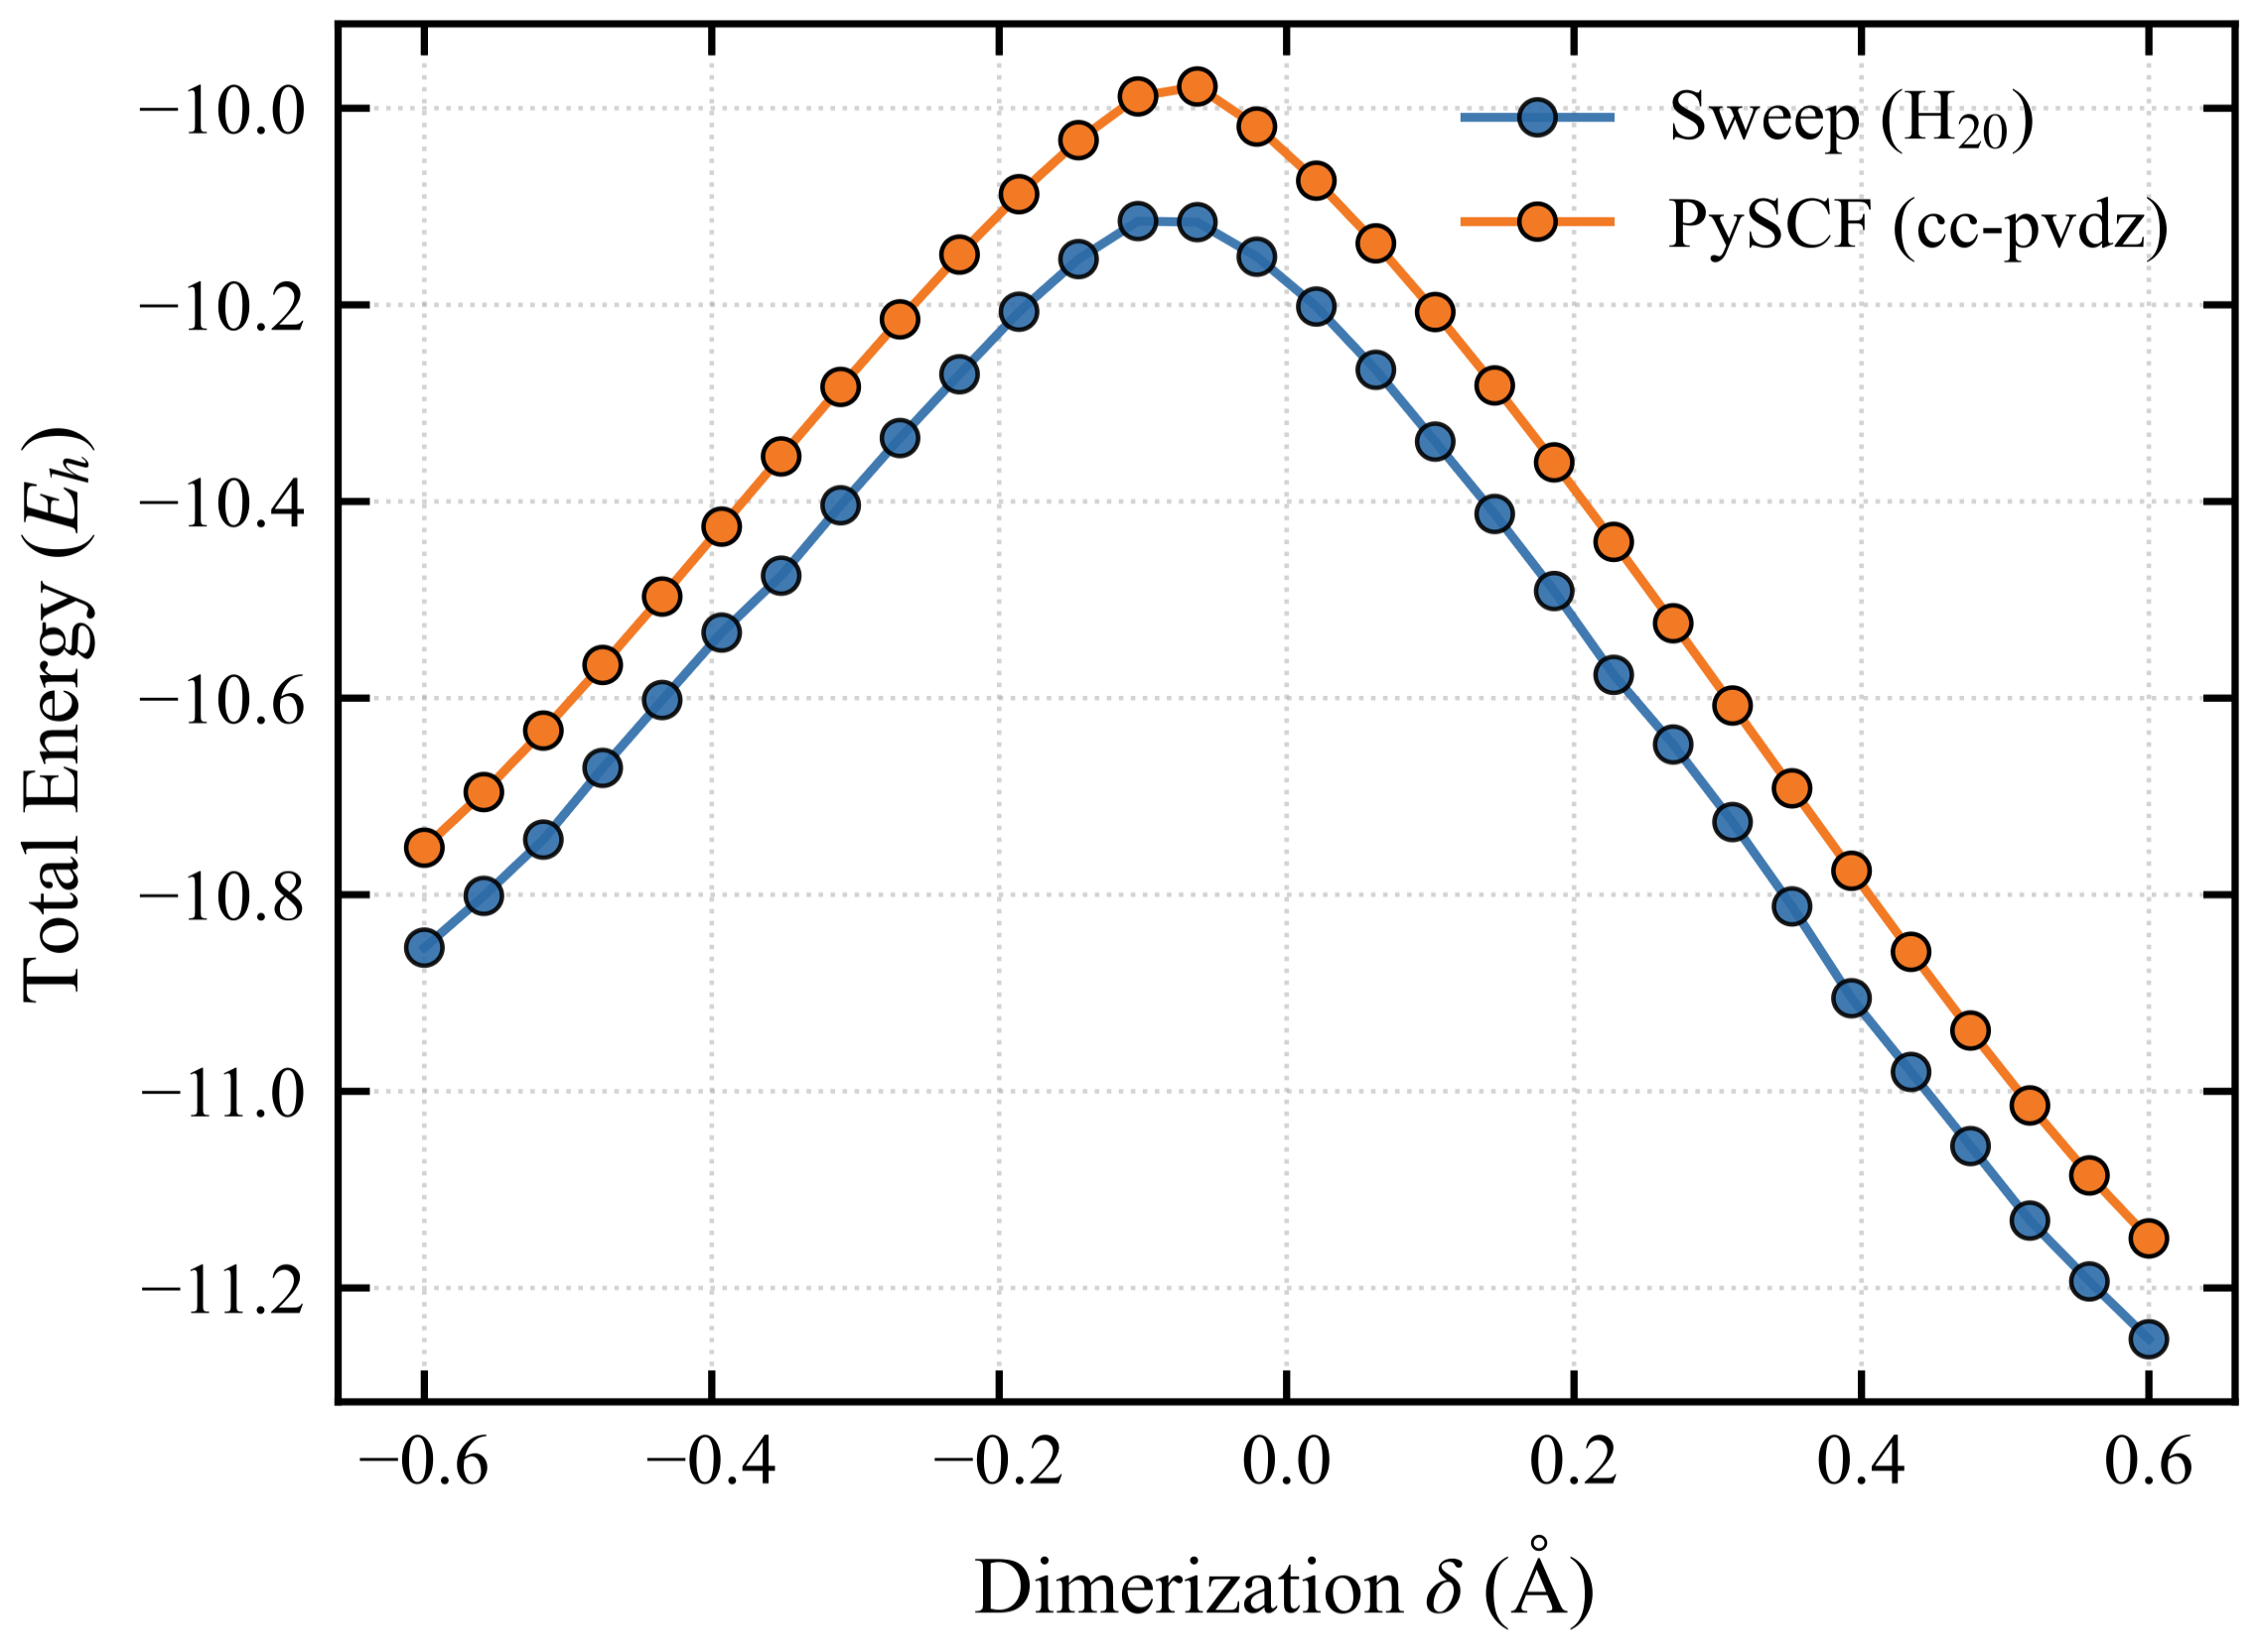
\includegraphics[width=0.7\textwidth]{fig/example_image_2.png} 
    \caption[$H_{20}$ 链的 Hartree-Fock 势能面基准测试]{%
      $H_{20}$ 链的 Hartree-Fock 势能面基准测试。
      图中展示了在一维氢原子链 ($N=20$) 模型中，体系总能量随晶格二聚化参数 $\delta$ 的变化关系。
      蓝色曲线（Sweep）为本研究开发的哈密顿量构建与自洽场求解程序的计算结果，
      橙色曲线（PySCF）为使用标准量子化学软件包（cc-pvdz 基组）计算的参考结果。
      结果显示，在测试的分子结构下，新基组在平均场下的表现已经优于传统高斯型轨道，为后续DMRG的应用奠定了坚实基础。}
    \label{fig:h20_hf_benchmark}
  \end{figure}
  
  最后，学校的高性能计算集群及服务器环境能够满足本研究中测试与计算的硬件需求。
  \section{研究计划进度安排及预期目标}
  \subsection{进度安排}
  正文内容
  \subsection{预期目标}
  正文内容

  % 以下是自动生成的开题报告部分的参考文献
  \printbibliography[heading=bibintoc, title={参考文献}]
\end{refsection}


\chapter{外文翻译}
% 实例
\section{实空间量子重整化群}
\noindent 原文标题：Real-Space Quantum Renormalization Groups\\
\noindent 来源：\textit{Phys. Rev. Lett.} \textbf{1992}, 68 (24), 3487–3490.
\subsubsection{翻译内容：}
从这个例子中吸取的教训是：在当前迭代中未被考虑的周围块（环境），其影响实际上等效于对当前块施加了多种变化的边界条件。因此，任何在块上仅使用单一特定边界条件的方法，所生成的一组态在某种意义上都是“不完备”的。而且这种不完备性很难通过保留更多的态或应用微扰修正来消除。
\section{原文标题翻译}
\noindent 原文标题：[to be filled]\\
\noindent 来源：\textit{Journal name}. \textbf{year}, other infomation.
\subsubsection{翻译内容：}
正文内容
\section{原文标题翻译}
\noindent 原文标题：[to be filled]\\
\noindent 来源：\textit{Journal name}. \textbf{year}, other infomation.
\subsubsection{翻译内容：}
正文内容


\chapter{外文原文}
% 实例
\section{实空间量子重整化群}
\noindent \textbf{Article Title:} Real-Space Quantum Renormalization Groups.\\
\noindent \textbf{Authors:} White, S. R.; Noack, R. M.\\
\noindent \textbf{Source:} \textit{Phys. Rev. Lett}. \textbf{1992}, 68 (24), 3487–3490.

\subsubsection{Original Texts:}

The lesson to be learned from this example is that the influence of the surrounding blocks not taken into account in the current iteration is to effectively apply a variety of boundary conditions to the current block. Hence, any approach using one set of boundary conditions on a block generates a set of states which is in some sense 'incomplete,' and it is very difficult to correct this incompleteness by keeping many states or by applying perturbative corrections.
\section{原文标题翻译}
\noindent \textbf{Article Title:} [title to be filled].\\
\noindent \textbf{Authors:} [Author name]\\
\noindent \textbf{Source:} \textit{Journal name}. \textbf{year}, other information.

\subsubsection{Original Texts:}
[text to be filled]
\section{原文标题翻译}
\noindent \textbf{Article Title:} [title to be filled].\\
\noindent \textbf{Authors:} [Author name]\\
\noindent \textbf{Source:} \textit{Journal name}. \textbf{year}, other information.

\subsubsection{Original Texts:}
[text to be filled]

\end{document}
